%%% This Beamer example was created by LianTze Lim, April 2017.

%%%% This is a VERY simple and minimalistic beamer theme,
%%%% even reminiscent of marker pens on transparencies!
%%%% It mimics the look of the "seminar" package, which
%%%% can only be used with plain TeX.
%%%% There are also some comments and example to show how
%%%% to customise various elements, e.g. the font and colours.

\documentclass[12pt]{beamer}
%% If you'd like the default font size to be even larger, use 14pt or 17pt; these are supported by Beamer.

\graphicspath{{Figures/}{Figures}}

%%%%%%%%%%%%%%%%%%%%%%%%%%%%%%%%%%%%%%%%%
% These lines should usually go into a .sty file,
% but I'll leave them here so that it's easier to
% see how to customise a Beamer theme.
% Remember, the Beamer manual is your friend!!
% http://texdoc.net/pkg/beamer
%
%% So if your re-definitions have a @ somewhere, you
%% _MUST_ put a \makeatletter before these lines and then
%% \makeatother after them. This trick can only be done
%% in the preamble! BUT if you're doing these re-definitions
%% in a .sty file (so that you \usepackage it later), you
%% don't need the \makeatletter and \makeatother.
\makeatletter

%% Set the left and right margins
\setbeamersize{text margin left=1em,text margin right=1em}

%% FONTS
\setbeamerfont{title}{series=\bfseries,size=\LARGE}
\setbeamerfont{subtitle}{series=\bfseries,size=\Large}
\setbeamerfont{frametitle}{series=\bfseries,size=\small}
\setbeamerfont{block title}{series=\bfseries,size=\normalsize}
\setbeamerfont{footline}{size=\small}

%% COLOURS
%% If you'd like everything to have the same colour
\usebeamercolor{structure}
\setbeamercolor{normal text}{fg=structure.fg}

%% Add a line after the frametitle
\addtobeamertemplate{frametitle}{}{\vspace*{-1ex}\rule{\textwidth}{1pt}}

%% Use circular discs as itemized list markers;
%% there's an existing option in Beamer for it so I'll use it
\setbeamertemplate{itemize items}[circle]

%% Remove default navigation symbols (We'll add the ones we need in the footline
\setbeamertemplate{navigation symbols}{}


%% And before the footline... actually we'd like to re-define
%% the footline
\setbeamertemplate{footline}{%
   %% Beamer headlines and footlines are always full-paperwidth, so if you want the horizontal line to
   %% not span it entirely you'll need to do a bit of arithmetic
   \centering
   \begin{minipage}{\dimexpr\paperwidth-\beamer@leftmargin-\beamer@rightmargin\relax}
   \centering
   \rule{\linewidth}{1pt}\vskip2pt
   \usebeamerfont{footline}%
   \usebeamercolor{footline}%
   %% The frame number smack in the middle
   \hfill\insertframenumber/\inserttotalframenumber
   \hfill%
   %% ONLY the navigation symbols we want at the far right.
   %% We use an \llap so that it takes up zero width, and doesn't throw the page number off-centre!
   \llap{\insertframenavigationsymbol\insertbackfindforwardnavigationsymbol}\par
   \end{minipage}\vskip2pt
}

\setbeamercolor{block title alerted}{fg=white,bg=brown}

\makeatother
%%%% END STYLE CUSTOMISATION %%%%%%%%%%%%

\usepackage[english]{babel}
\usepackage[latin1]{inputenc}
\usepackage[T1]{fontenc}
\usepackage{graphicx}

\usepackage{subcaption}

\usepackage{times}

\usepackage{graphics}
%\usepackage[draft]{graphics}

\usepackage{xspace}
\usepackage{amsmath}
\usepackage{bm}
\usepackage{pgfpages}
\usepackage{fancybox}
\usepackage{threeparttable}
\usepackage{bbding}
\usepackage{verbatim}
\usepackage{booktabs}

\usepackage{natbib}
\bibpunct{(}{)}{;}{a}{}{,}

\newcommand{\pkg}[1]{{\normalfont\fontseries{b}\selectfont #1}}
\let\proglang=\textsf
\let\code=\texttt

\newcommand{\btheta}{ \mbox{\boldmath $\theta$}}
\newcommand{\bbeta}{ \mbox{\boldmath $\beta$}}
\newcommand{\balpha}{ \mbox{\boldmath $\alpha$}}
\newcommand{\by}{ \mbox{\bf y}}
\newcommand{\bY}{ \mbox{\bf Y}}
\newcommand{\bX}{ \mbox{\bf X}}
\newcommand{\bH}{ \mbox{\bf H}}
\newcommand{\bI}{ \mbox{\bf I}}


\title{Introduction to disease mapping - Part 2}
\subtitle{}
\author{Bayesian modelling for spatial and spatio-temporal data}
\institute{MSc in Epidemiology}
\date{Week 6}


\begin{document}

\begin{frame}[t]
  \titlepage
\end{frame}


\begin{frame}
    \frametitle{Aims of disease mapping}
Disease maps used variously for:
\begin{itemize} \setlength\itemsep{\fill}
\item Descriptive purposes: to summarise spatial and spatio-temporal variation in disease risk $\rightarrow$ a visual summary of geographical risk;
\item To generate etiological hypotheses: informal examination of disease maps with exposure maps (followed by formal examination via spatial regression);
\item For surveillance, to highlight areas at apparently high risk;
\item To aid policy formation and resource allocation.
\end{itemize}
\end{frame}
%%%%%%%%%%%%%%%%%%%%%%%%%%%%%%%%%%%%%%%%%%%%%%%%%%%%%%%%%%%%%%%%

\begin{frame}
    \frametitle{What to map?}
\begin{itemize} \setlength\itemsep{\fill}
\item \textbf{Mortality}
    \begin{itemize} \setlength\itemsep{\fill}
    \item  most readily available source of data for all diseases
    \item  should be complete and relatively accurate
    \end{itemize}
\item \textbf{Morbidity}
	\begin{itemize} \setlength\itemsep{\fill}
    \item  \textbf{Incidence}, that is the number of new cases within a specific time frame
    \begin{itemize} \setlength\itemsep{\fill}
    \item  incidence data usually routinely available for cancer registries
   % \item  may be more sensitive to effects of exposure (shorter time lag between exposure and event compared to mortality)
    \end{itemize}
	\item \textbf{Prevalence}, that is the total number of existing cases over specific time frame
    \begin{itemize} \setlength\itemsep{\fill}
    \item  available from registries and hospital admissions
    \end{itemize}
\end{itemize}
    \end{itemize}
\end{frame}
%%%%%%%%%%%%%%%%%%%%%%%%%%%%%%%%%%%%%%%%%%%%%%%%%%%%%%%%%%%%%%%%
\begin{frame}
    \frametitle{Geographical scales}
Disease mapping may be carried out at a variety of geographical scales:
\begin{itemize}
\item \vfill \textbf{International}:
    \begin{itemize}
    \item Comparisons between countries, e.g World Health Organization (WHO) or International Agency for Research on Cancer (IARC) reports
    \end{itemize}
\item \vfill \textbf{National}:
    \begin{itemize}
    \item Comparisons between e.g. regions, districts
    \item  \vfill Most published disease atlases fall into this category
    \end{itemize}
\item \vfill \textbf{Small area studies}
    \begin{itemize}
    \item \vfill Sub-national scale, e.g. wards, municipalities
   % \item \vfill Becoming increasingly common as data and methods improve
    \end{itemize}
\end{itemize}
\end{frame}

%%%%%%%%%%%%%%%%%%%%%%%%%%%%%%%%%%%%%%%%%%%%%%%%%%%%%%%%%%%%%%%%
%\begin{frame}
% \frametitle{International scale: lung cancer mortality rates - worldwide, 2018}
%Estimated age-standardized rates (World) per 100,000 (males, all ages).
%\begin{figure}
%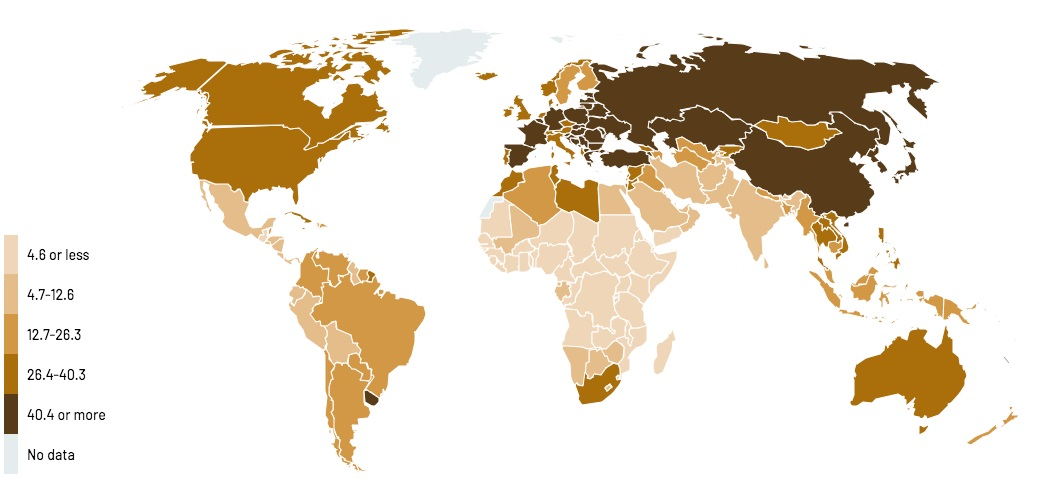
\includegraphics[scale=0.50]{LungCancer_Male2018.jpg}
%\end{figure}
%\tiny source: Ferlay J, Ervik M, Lam F. et al. Cancer today. Lyon France. IARC. Available at \url{https://canceratlas.cancer.org/the-burden/lung-cancer/}
%{\small
%\begin{itemize}
%  \item Large international differences in mortality rates of lung cancer, potentially explained by differences in the prevalence of smoking
%\end{itemize}
%}
%\end{frame}

%%%%%%%%%%%%%%%%%%%%%%%%%%%%%%%%%%%%%%%%%%%%%%%%%%%%%%%%%%%%%%%%

%\begin{frame}
% \frametitle{National scale: lung cancer mortality and nitrogen dioxide (NO$_2$) exposure - England}
%Maps of lung cancer standardized morbidity ratios (SMRs) (2011-2012) and NO$_2$ (2001) at district level
%\begin{figure}
%\begin{tabular}{cc}
%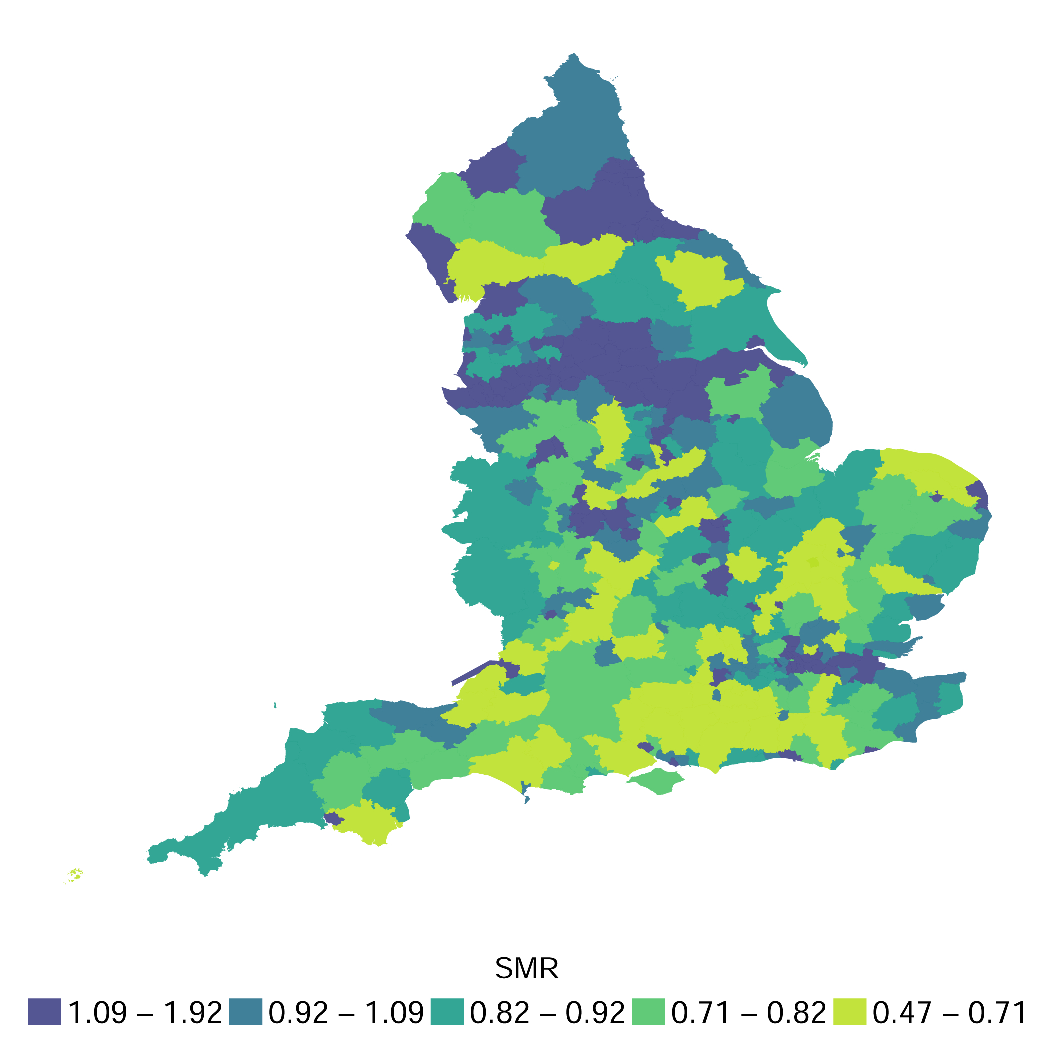
\includegraphics[width=5 cm]{Map_SMR.pdf}&
%\includegraphics[width=5 cm]{Map_NO2.pdf}\\
%\end{tabular}
%\end{figure}

%{\small
%\begin{itemize}
%  \item Is there a positive association?
%\end{itemize}
%}
%\end{frame}

%%%%%%%%%%%%%%%%%%%%%%%%%%%%%%%%%%%%%%%%%%%%%%%%%%%%%%%%%%%%%%%%
\begin{frame}
    \frametitle{Small area case study: lung cancer incidence in males - England and Wales}
Map of the SMRs for the period 1985-2009 at ward level
\begin{columns}
\column{2.5in}
\begin{figure}
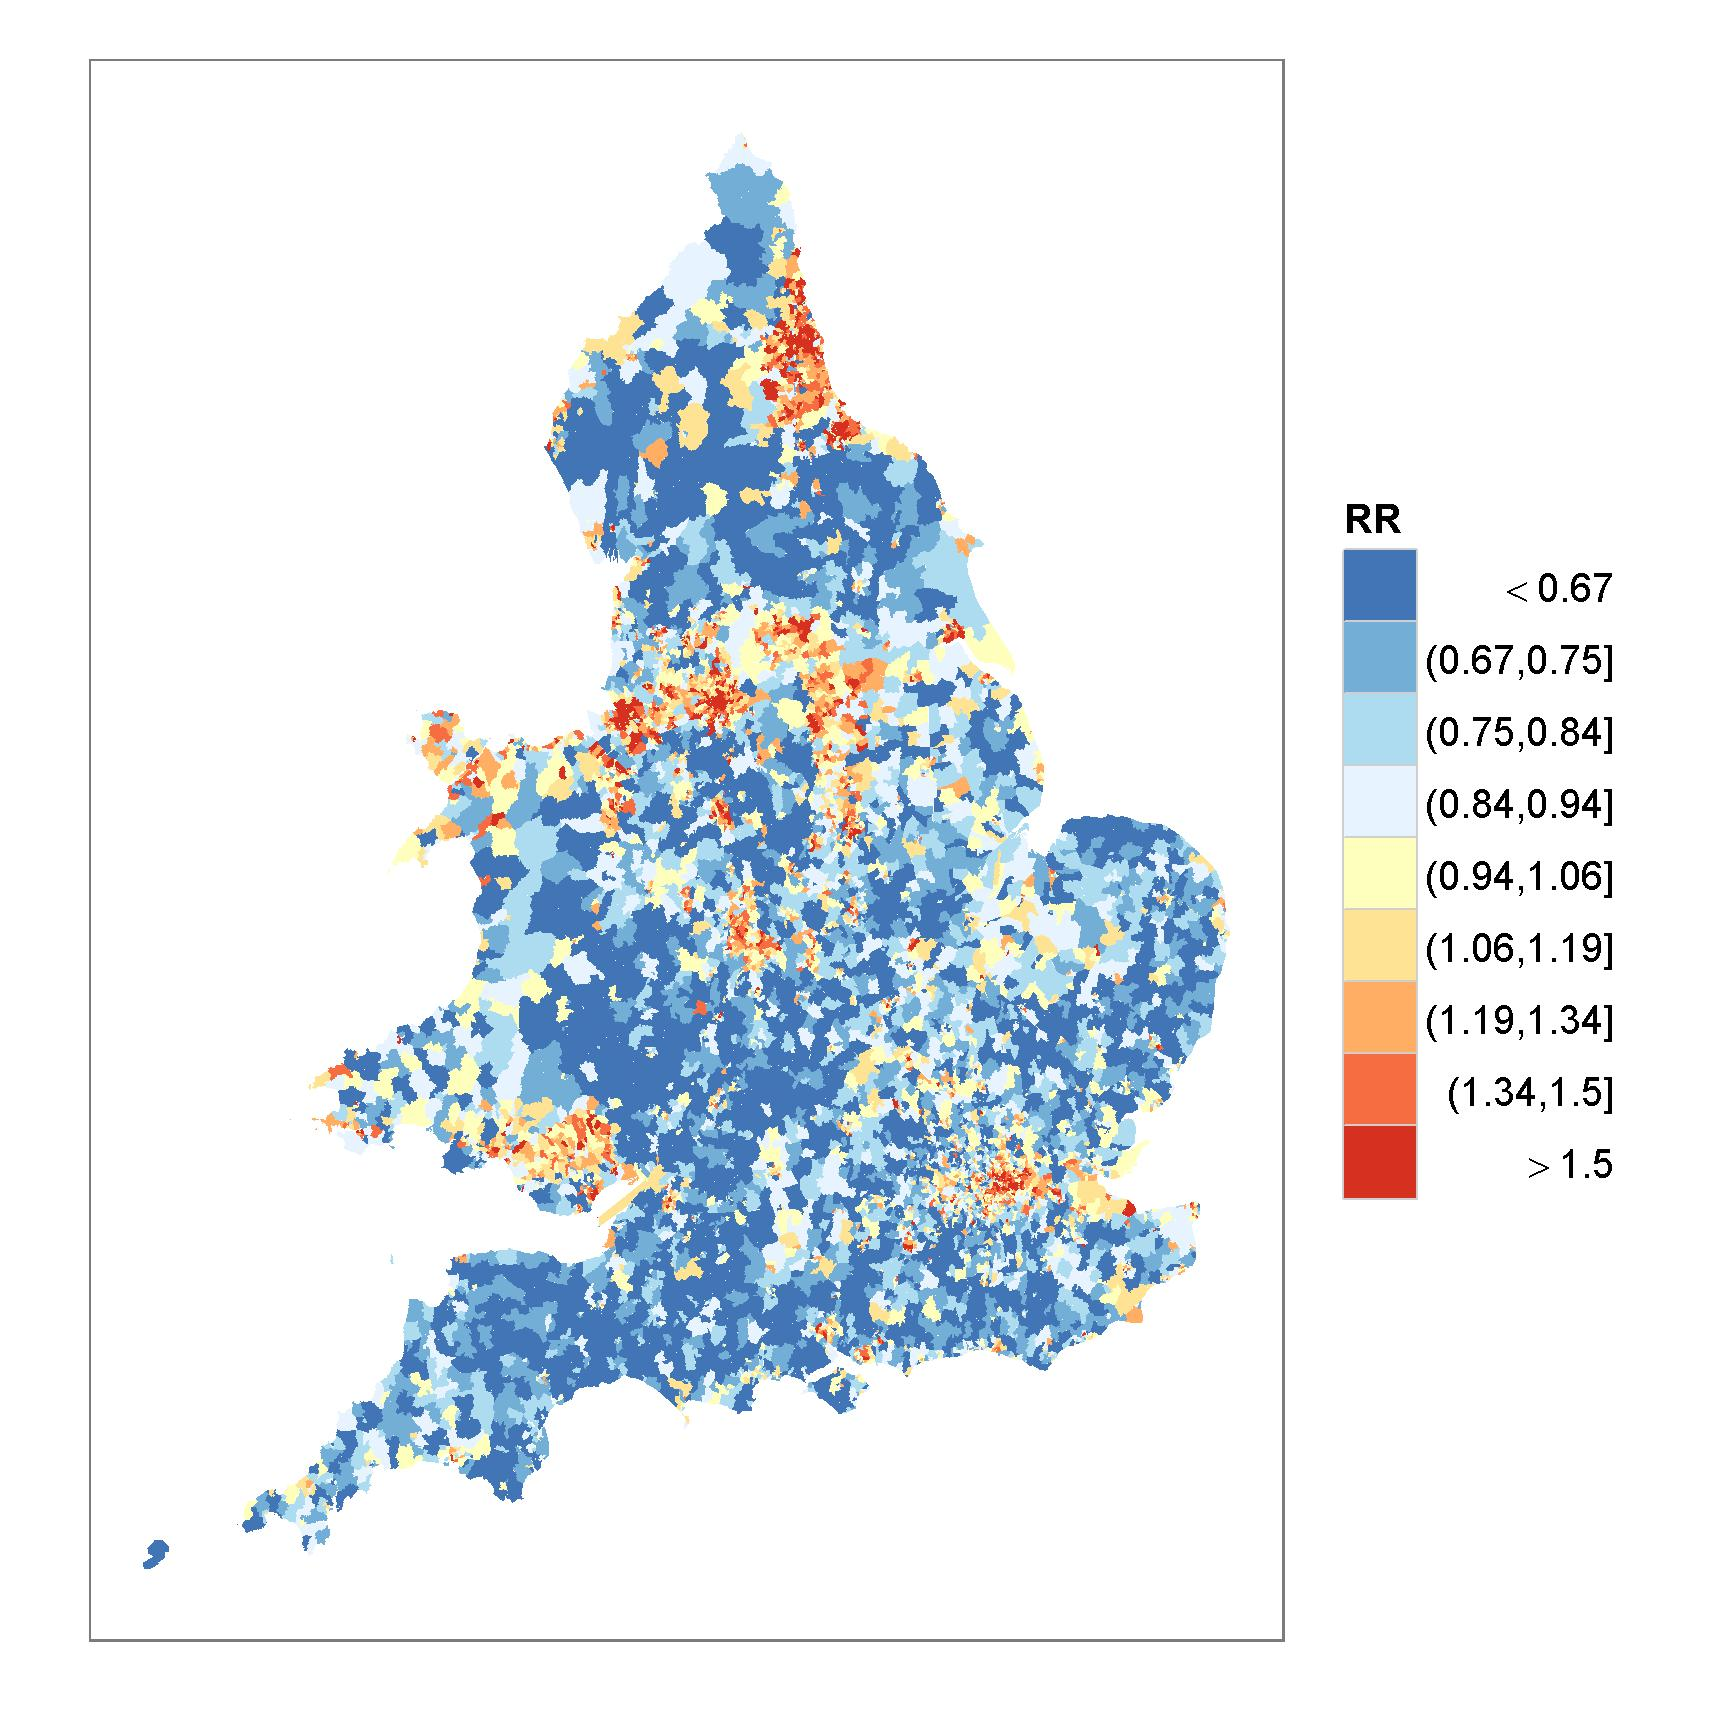
\includegraphics[scale=0.35]{Lungmales_SMRmap.jpg}
\end{figure}
\vspace{-10pt}
{\tiny
\begin{table}
    \begin{tabular}{|l|l|l|l|l|l|}
        \hline
        ~   & Min  & Q1    & Median & Q3    & Max    \\ \hline
        O   & 0    & 26    & 47     & 84    & 456    \\
        E   & 3.25 & 32.14 & 53.60  & 82.47 & 390.49 \\
        SMR & 0    & 0.70  & 0.89   & 1.13  & 2.63   \\
        \hline
    \end{tabular}
\end{table}
}
\column{2.0in}
\begin{itemize}
  \item \vfill Is the variability real or simply reflecting unequal $E_i$s?
  \item \vfill Have the highlighted areas truly a raised relative risk?
\end{itemize}
\end{columns}
\end{frame}

%%%%%%%%%%%%%%%%%%%%%%%%%%%%%%%%%%%%%%%%%%%%%%%%%%%%%%%%%%%%%%%%

\begin{frame}
    \frametitle{Problems with mapping SMRs}
\begin{itemize} \setlength\itemsep{\fill}
\item It is common practice to map SMRs, however:
    \begin{itemize}
    \item  $\hbox{SMR}_i$ very imprecise for rare diseases and/or areas with small populations,
    \item  For the model $O_i \sim \hbox{Poisson}(\lambda_i E_i)$, the MLE is $\hbox{SMR}_i=\frac{O_i}{E_i}$, and its estimated variance is $\hat{\hbox{Var}}(\hat{\lambda}) =  \frac{O_i}{E_i^2}$,
    \item  areas with small $E_i$ have high associated variance.
    \end{itemize}
\vspace{0.2cm}
\item  SMR in each area is estimated independently:
    \begin{itemize}
    \item[$\rightarrow$] makes no use of risk estimates in other areas of the map, even though these are likely to be similar.
    \end{itemize}
\vspace{0.2cm}
\item[$\Rightarrow$] Highlights extreme risk estimates based on small numbers, thus risks tend to be unstable.
\vspace{0.2cm}
\item[$\Rightarrow$] Ignores possible spatial correlation between disease risk in nearby areas due to possible dependence on spatially varying risk factors.
\end{itemize}
\end{frame}

\begin{frame}
\frametitle{Smoothing}
\begin{itemize} \setlength\itemsep{\fill}
\item  One method for addressing these problems and reducing the noise in rates or risks associated with geographical areas is the \alert{`spatial smoothing'}.
\item \vfill The basic idea is to \alert{borrow information} from neighbouring areas to produce a better (i.e. more stable and less noisy) estimate of the risk associated with each area and thus separate out the signal from the noise.

\item  We will use Bayesian `smoothing' estimators in a hierarchical formulation:
\begin{itemize}
\item  \alert{Poisson-lognormal model: non-spatial (global) smoothing}
\item  \alert{Poisson-lognormal spatial model: spatial and non-spatial smoothing}
\end{itemize}
\end{itemize}
\end{frame}

\begin{frame}
    \frametitle{Poisson-lognormal model (non-spatial smoothing)}
Model:
    %\vspace{-10pt}
\begin{eqnarray*}
O_i & \sim & \hbox{Poisson}(\lambda_i E_i) \\
%\mu_i=\lambda_i E_i \\
\log(\lambda_i) & = & \alpha + \theta_i\\
\theta_i & \sim  & \hbox{Normal}(0, \sigma_{\theta}^2) \\
\alpha &\sim & \hbox{Normal}(0,10^4)\\
\end{eqnarray*}
\vspace{-10pt}
{\footnotesize
\begin{itemize}\setlength\itemsep{\fill}
\item $O_i$ and $E_i$ are observed and expected number of cases in area $i$
\item $\boldsymbol{\theta}=(\theta_1, \dots, \theta_N)$ are \emph{exchangeable parameters} and each $\theta_i$ follows the same prior distribution, but, in addition, we assign a prior distribution (hyperprior) to the unknown parameter of that prior distribution:
    $1/\sigma^2_{\theta} \sim \text{Gamma}(1, 0.01)$ %$$\sigma_{\theta}^2 \sim \text{Inverse Gamma}(1, 0.01) \Leftrightarrow \tau_{\theta} \sim \text{Gamma}(1, 0.01)$$
%\item $\sigma_{\theta}^2$ is between-area variance
\end{itemize}
}
\vspace{-5.5pt}
\par\noindent\rule{\textwidth}{0.4pt}
\scriptsize{Recall: the reciprocal of the variance is the precision $ 1/\sigma^2_{\theta} = \tau_{\theta} $}
%\scriptsize{Recall $Y \sim \text{Inverse Gamma}(a,b) \Leftrightarrow   X = \frac{1}{Y} \sim \text{Gamma}(a,b), \hbox{E}(X) = \frac{a}{b}, \hbox{Var}(X)= \frac{a}{b^2}$}
\end{frame}

\begin{frame}
\frametitle{Parameter interpretation}
\begin{itemize} \setlength\itemsep{\fill}
\item  $\lambda_i=\exp (\alpha +  \theta_i)$: unknown RR in area $i$ compared with expected risk based on age and sex of population
  \item  Parameter $\alpha$: mean log relative risk, i.e. overall risk in the region of study
  \item  Parameters $\theta_i$: {\bf area-specific random effects} to capture region-wide \emph{heterogeneity}. They take into account the extra-Poisson variability, i.e.  \alert{overdispersion}, in the log-relative risks. The excess variation can be due to:
  \begin{itemize} \setlength\itemsep{\fill}
    \item errors in numerators (observed counts) and denominators (expected counts)
    \item unobserved or unknown risk factors (confounders)
  \end{itemize}
  \item  residual RR = $\exp (\theta_i)$
  \item $\sigma_{\theta}^2$: is between-area variance and controls the magnitude of the $\theta_i$ %reflects the amount of extra-Poisson variation in the data
\end{itemize}
\end{frame}




\begin{frame}
    \frametitle{Mapping smoothed \emph{vs} raw estimates of $\lambda_i$}
    \begin{center}
    Lung cancer incidence in males, 1985-2009, England and Wales
        \scalebox{0.65}{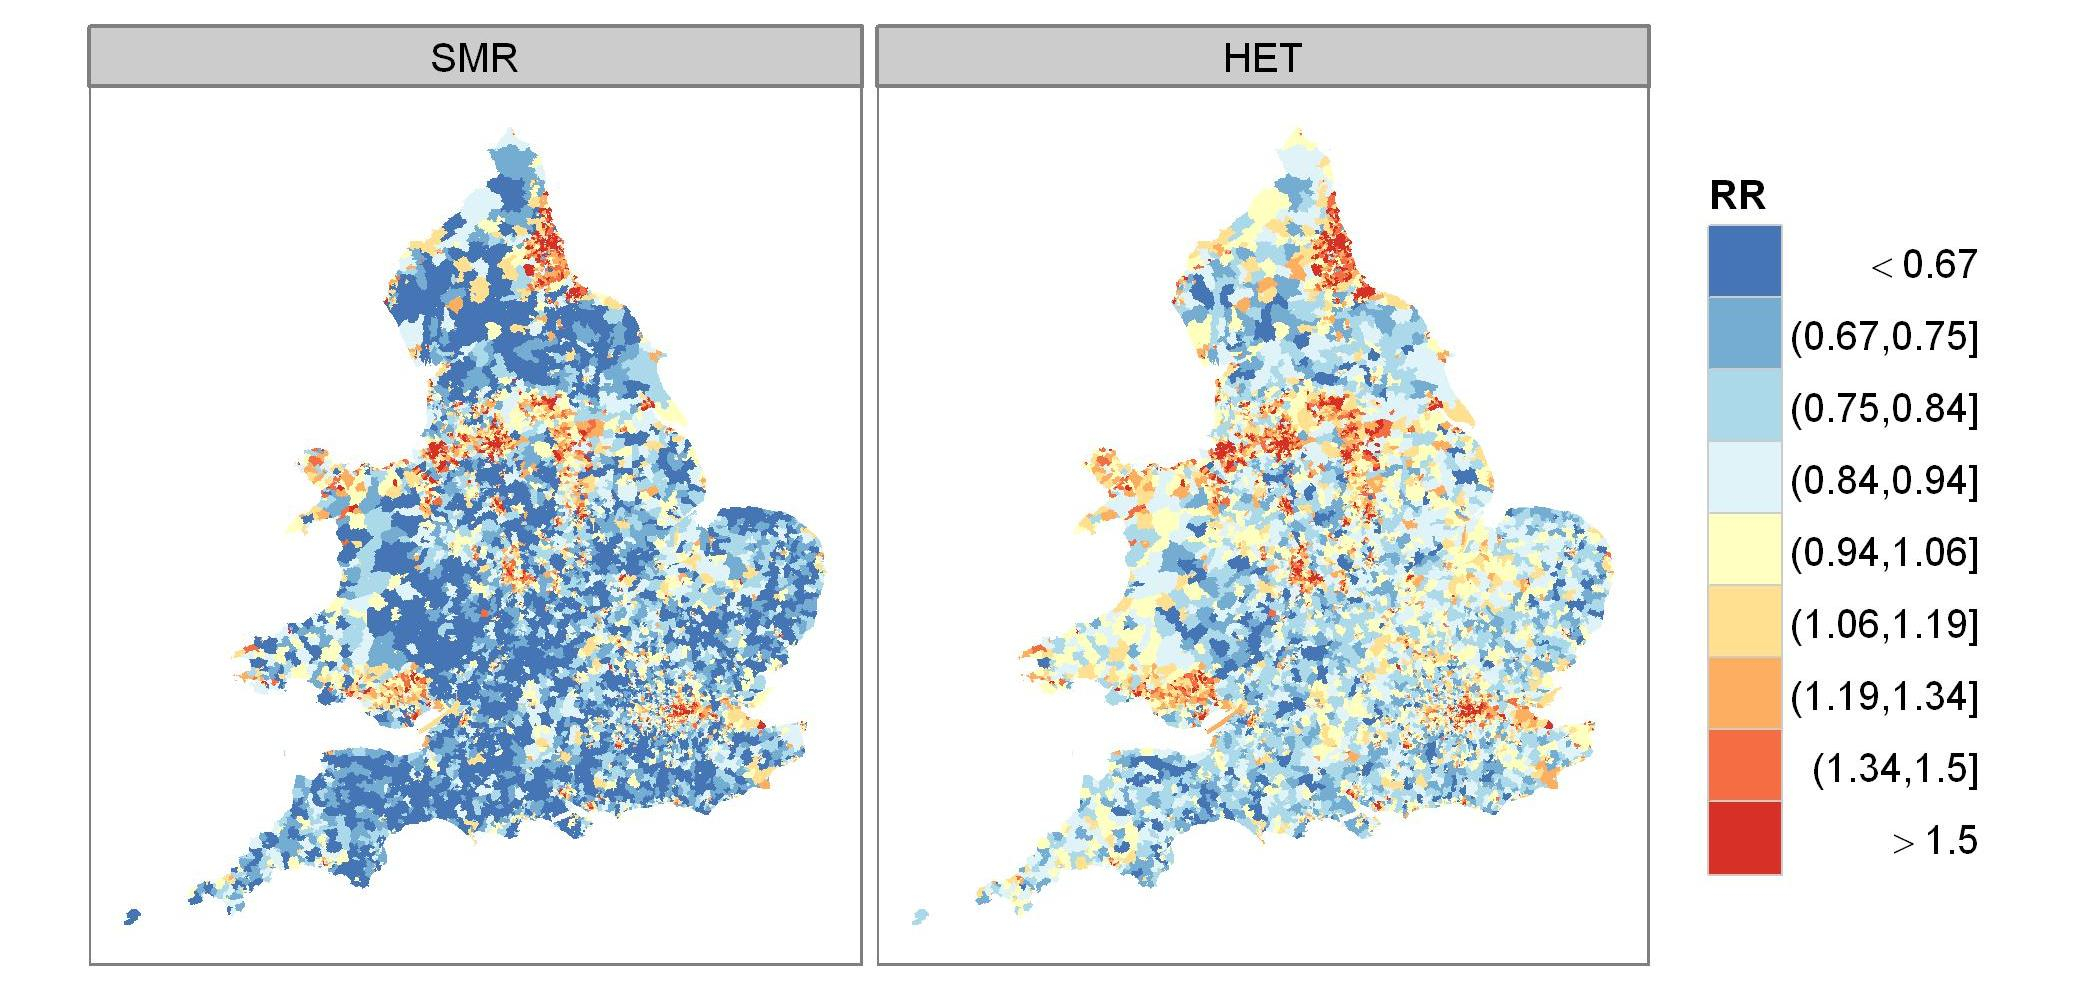
\includegraphics{Lungmales_SMRHETmap.jpg}}\\
        SMRs and non-spatially smoothed RRs
    \end{center}

\par\noindent\rule{\textwidth}{0.4pt}
\footnotesize{Note: It is important to keep the same cut points when comparing maps}
\end{frame}


\begin{frame}
SMRs versus non-spatially smoothed RRs in selected areas for lung cancer incidence in males, 1985-2009, England and Wales
\begin{center}
        \scalebox{0.25}{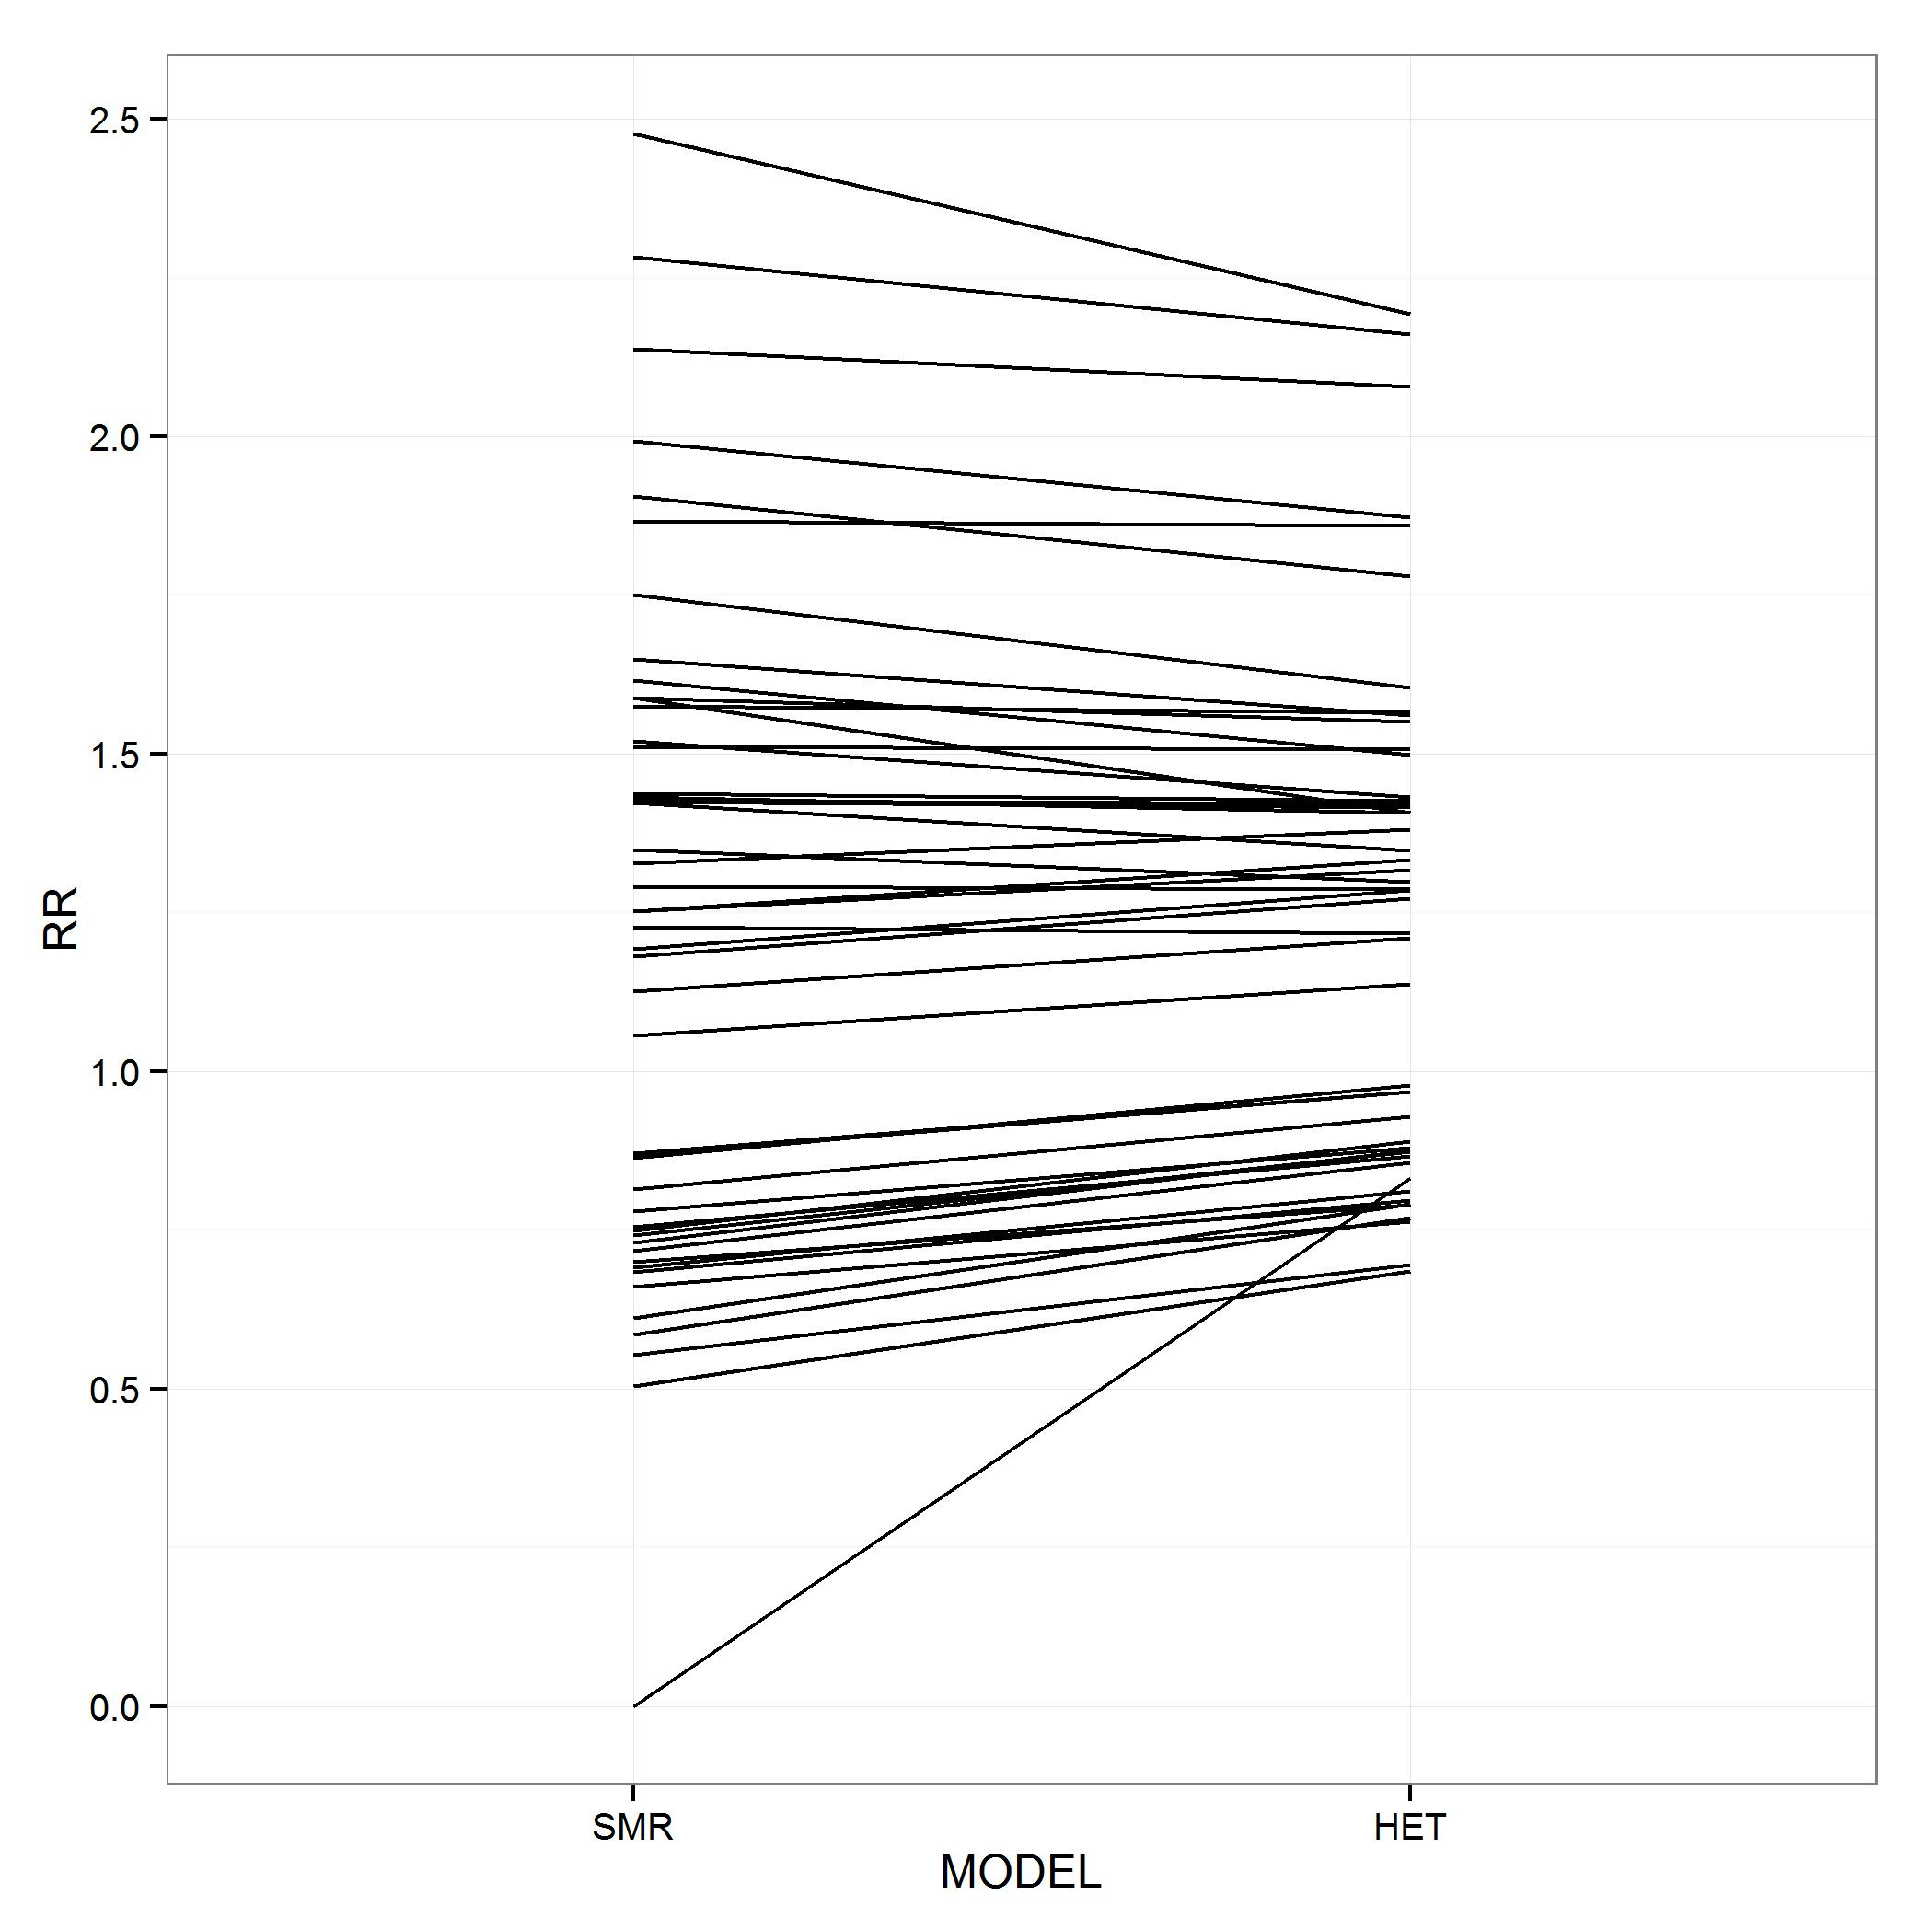
\includegraphics{Lungmales_SMRHETshrinkage.jpg}}\\
\end{center}

\vspace{-0.1cm}
\begin{itemize} \setlength\itemsep{\fill}
\item Shrinkage towards the mean when using a hierarchical model
\item Posterior mean and 95\% credible intervals (CI) = 1.0 (95\%CI: 1.09-1.1) % 0.094 (0.091-0.098) on log scale
%$\sigma_v^2$ = between-area variance of log relative risk of lung cancer\\
\end{itemize}
\end{frame}


\begin{frame}
\frametitle{Binomial framework}
  \begin{itemize} \setlength\itemsep{\fill}
\item For more common diseases, Binomial model may be preferred
	$$O_i \sim \hbox{Binomial}(p_i ,n_i)$$
where
  \begin{itemize} \setlength\itemsep{\fill}
	\item $n_i$ = population at risk
	\item $p_i$ = probability of disease
  \end{itemize}
\item $\hbox{logit}(p_i) = \alpha + \theta_i$
\item Parameter of interest: Odds ratio $\hbox{OR}_i = \exp(\alpha + \theta_i)$
\end{itemize}
\end{frame}


\begin{frame}
\frametitle{A few notes on ecological bias [1]}
\begin{itemize} \setlength\itemsep{\fill}
\item In our module, we work often with aggregated data
\item Aggregation has implications for the type of inference that are possible
\item Ecological inference is the process where aggregated data are used to infer individual level relationships. Reasons:
\begin{itemize}
  \item individual data are not available for confidentiality reasons
  \item individual data are not reliable or too expensive to be collected
\end{itemize}
\item \alert{Ecological (or aggregation) bias in the difference between the estimates of relationships obtained using grouped data and those estimates obtained using individual data}
     (e.g. the association observed at the area level do not hold for the individuals within areas).
\end{itemize}
\end{frame}

\begin{frame}
\frametitle{A few notes on ecological bias [2]}
\begin{itemize} \setlength\itemsep{\fill}
\item Ecological bias can manifest itself in a variety of ways and results in an information loss (e.g. it can be due to a model specification bias that arises because a nonlinear risk model changes its form under aggregation). Researchers should specify the conditions under which the estimates are reasonable.
\item The converse, using individual level estimates uncritically to infer group level relationships (ignoring the possibility of group level or contextual effects) is called as \alert{atomistic or individualistic fallacy}.
\end{itemize}
%e.g. bias in resulting health risks may occur due to the aggregation of non-linear model
\end{frame}

\begin{frame}
\frametitle{Reference}
\begin{itemize} \setlength\itemsep{\fill}
\item Banerjee S., Carlin B.P, Gelfand A. (2014), Hierarchical Modeling and Analysis for
Spatial Data. (2nd ed.) CRC Press - Section 6.4.1 (partially Section 6.4.3.2)
\item Haining R., Guangquan L. (2020), Modelling Spatial and Spatial-Temporal Data. A Bayesian Approach, CRC Press
- Section 7.4.2
\end{itemize}
\end{frame}

\end{document} 